\documentclass[12pt]{article}
\usepackage{graphicx}
\graphicspath{ {./images/} }
%encoding
%--------------------------------------
\usepackage[T1]{fontenc}
\usepackage[utf8]{inputenc}
%--------------------------------------

%Portuguese-specific commands
%--------------------------------------
\usepackage[portuguese]{babel}
%--------------------------------------

%Hyphenation rules
%--------------------------------------
\usepackage{hyphenat}
\hyphenation{mate-mática recu-perar}
%--------------------------------------
\usepackage{enumerate}

\usepackage{hyperref}
\hypersetup{
    colorlinks=true,
    linkcolor=blue,
    urlcolor=blue,
}

\urlstyle{same}


\begin{document}

\tableofcontents


\section{Introdução}

O processo seletivo deixou de constituir apenas um meio de contratação de mão de obra em que o maior beneficiado final é o contratante. Na sociedade contemporânea, difunde-se de forma exponencial a cultura de organizações voltadas à valorização do bem-estar do empregado desde a etapa de seleção desse, em que seus aspectos psicológicos e sociaisrecebem uma maior atenção e cuidado por parte dos empregadores. Assim, observa-se que hoje há uma tendência que as organizações valorizem muito mais o indivíduo e suas necessidades, e não apenas suas qualificações técnicas e acadêmicas.

Diante de tal realidade, esse trabalho realiza análise crítica de um processo seletivo que ocorreu no início de 2019 à empresa \emph{Conduent} do Brasil para o cargo de Analista de Suporte Técnico Bilíngue Júnior, no qual o objetivo era prestar suporte de software via telefone aos produtos de uma das maiores empresas de dispositivos \emph{mobile} e \emph{desktop} do mundo.

Essa análise crítica trata, desde o primeiro contato da empresa via plataforma de currículos online, até a efetivação da contratação. Por isso, percorre o total de oito etapas que constituíram o processo seletivo realizando argumentação acerca da validade e/ou efetividade da etapa em questão através da análise do contexto do candidato, da empresa e de contextos mais globais - que podem abarcar questões que tangem o mercado de trabalho, um certo nicho da sociedade, etc.

Dessa maneira, tem-se como foco verificar se a maneira pela qual o processo seletivo foi conduzido proporcionou aos candidatos uma experiência que valorizasse sua existência enquanto seres humanos e profissionais e assim contribuísse para que cada indivíduo atinja seus objetivos de autorrealização. 

Portanto, diante esse viés crítico, fatos, teorias e metodologias foram correlacionados a fim de dar embasamento a cada posicionamento.


\addcontentsline{toc}{section}{Unnumbered Section}
\section*{Unnumbered Section}

\url{ https://pt.overleaf.com/learn/latex/Table_of_contents}


% resumo em português
\setlength{\absparsep}{18pt} % ajusta o espaçamento dos parágrafos do resumo
\begin{resumo}

Este projeto tem como objetivo analisar detalhadamente as etapas do processo seletivo da empresa Conduent Brasil desde o registro do currículo até o estabelecimento do contrato. Também serão abordados tópicos como a avaliação da experiência dos funcionários na empresa e como ela enfrenta crises globais como a do COVID-19.    


\textbf
{Palavras-chaves}: processo seletivo. empresa.
\end{resumo}

% resumo em inglês
\begin{resumo}[Abstract]
 \begin{otherlanguage*}{english}
  This project aims to analyze in detail the steps of the Conduent Brasil's selective process since the registration of the curriculum to the contract establishment. There will be also topics like the evaluation of the employee's experience in the company and how it faces global crysis like COVID-19.

   \vspace{\onelineskip}
 
   \noindent 
   \textbf{Key-words}: selective process. company.
 \end{otherlanguage*}
\end{resumo}



\maketitle


\section*{Dos meios de candidatura}

A \emph {Conduent} possui duas principais maneiras pelas quais candidatos podem se candidatar a vagas: via plataformas de cadastro de currículo online - meio em que a empresa também divulga suas vagas, ou, via indicação de funcionários. Trataremos mais especificamente da primeira maneira, pois o processo seletivo sob análise se deu pelo site vagas.com, entretanto, é relevante colocar em perspectiva ambas as possibilidades pois elas já impactam na experiência do candidato. 

O processo online, que é o mais comum dentro da Conduent, ocorre através de diversos portais de emprego, dentre os quais:

\begin{itemize}
\item www.vagas.com.br
\item www.linkedin.com.br
\item www.indeed.com.br
\item www.glassdoor.com.br
\item www.catho.com.br
\end{itemize} 

Tal presença em alguns dos maiores sites de emprego do país gera enorme alcance à empresa e, como consequência, mais chances de candidatos às vagas. Esse é um ponto muito positivo da empresa: a facillidade de encontrar vagas associadas a seu nome nos mais diversos meios online.

Além disso, a divulgação de vagas na rede precede que os pré-requisitos e objetivos dentro da posição divulgada sejam muito bem definidos pela empresa, evitando, assim, que haja um desencontro de expectativas do profissional para com a organização e vice-versa. 

E observa-se que a diversidade  presente na internet é alcançada pela empresa, e tal como o Código de Conduta Empresarial da Conduent" afirma: 

\begin{quote}
A diversidade nos torna mais fortes, pois permite que possamos aproveitar completamente uma força de trabalho global rica em experiência, conhecimento e criatividade.
\end{quote}


Dessa forma, tessa pluraridade alcançada pela Conduent faz com que a divulgação de candidaturas online tenha mais um aspecto positivo. 

Já em relação a candidaturas por indicação, de maneira geral, podemos observar que manisfestam-se dois aspectos dessas: a diversidade alcançada pela empresa é consideravelmente reduzida, contudo, o perfil de profissional buscado tende a ser o mais próximo daquilo que a vaga demanda. 

O motivo disso pode ser constatado ao se considerar que o profissional que faz a indicação já possui algum nível de vivência na empresa, de sua cultura organizacional, dos desafios enfrentados diariamente e resultados esperados ao desempenhar sua função. Assim, ao conseguir transmitir para o futuro indicado de forma mais personalizada os pré-requisitos da vaga, existe aí uma tendência de que ele esteja mais consciente do que se esperar.  

De certo, é preciso considerar que existe a parcialidade daquele que indica durante a transmissão de informações sobre o ambiente da empresa e do nível de satisfação com o trabalho desempenhado nela. Devido a isso, apesar da tendência citada, pode ocorrer o efeito oposto em alguns candidatos - especialmente aqueles que estão mais emocionalmente ligados ao que lhes indica - e tenham expectativas desniveladas em relação a posição.

Em síntese, temos que a Conduent está muito presente no meio digital, logo, as candidaturas online são as mais comuns, e essas permitem que a empresa alcance um maior e mais diverso número de indivíduos, bem como divulgue de forma objetiva os pré-requisitos e objetivos da função. Em relação as candidaturas por indicação, nota-se que existe uma maior chance de encontrar candidatos mais aptos às funções, porém, com a ressalva de que a percepção daquele que já integra o quadro de funcionários passa a ter papel de grande influência.  
 
\section*{Canditadura online - realizada através do site www.vagas.com.br}
 
No site da empresa www.vagas.com.br, a Conduent disponibilizou a vaga de Suporte Técnico Júnior Bilíngue no primeiro semestre de 2019 com o foco em candidatos interessados em trabalhar com suporte técnico de software via telefone para uma grande empresa do ramo de dispositivos mobile e desktop. Por questões de  \emph {compliance}, o nome da empresa para a qual o serviço seria prestado não poderia ser divulgado. Contudo, algumas das principais informações disponibilizadas eram: 
 
  \begin{itemize}
\item Quanto ao objetivo:
	\begin{enumerate}
	\item Oferecer atendimento para resolução problemas de software em dispositivos mobile 	visando proporcionar a melhor experiência ao cliente.
	\end{enumerate}
\end{itemize}


 \begin{itemize}
\item Quanto aos pré-requisitos:
	\begin{enumerate}
   	\item Possuir ensino médio completo;
	\item Inglês intermediário;
   	\item Ter facilidade com tecnologia; 
   	\item Ser criativo e proativo na solução de problemas; 
   	\item Ter boa desenvoltura para lidar com situações de conflito. 
	\end{enumerate}
\end{itemize}

E neste processo seletivo, a empresa responsável pelo processo de entrevistas foi a \emph {AgileOne} - empresa multinacional focada em oferecer serviços da área de Recursos Humanos para outras companhias.

Ao identificar candidatos em potencial, o primeiro contato  \emph {AgileOne} após indicação de interesse na vaga foi através de mensagem automática  via plataforma do vagas.com. Na mensagem, além do agradecimento pelo interesse, foi solicitada a realização de dois testes ainda dentro da plataforma: um de português e outro de inglês, ambos com cerca de 30 questões.

Tal contato via plataforma do vagas.com é positivo, pois o sistema notifica o candidato ao receber mensagens de recrutadores e isso facilita o retorno desse à empresa o quanto antes possível. Por consequência, as chances de que a oportunidade seja perdida diminuem consideravelmente quando comparado a empresas que tentam realizar contato inicial diretamente por telefone ou e-mail - meios que não necessariamente estarão a todo o momento voltados a verificação da resposta de empresas, diferentemente da plataforma especializada.

Além disso, temos que os testes online, ao considerar os candidatos que atendam os pré-requisitos estabelecidos na vaga de ensino médio completo e inglês intermediário, podem ser classificados como fáceis. Contudo, ao se levar em consideração a especificidade de que o trabalho demandaria o entendimento de um inglês mais técnico, essa facilidade não necessariamente representa algo positivo. 

Os candidatos com um nível de domínio da língua inglesa abaixo do necessário podem obter bons resultados devido ao teste simples e genérico da plataforma, mas como consequência, ao prosseguir às próximas etapas do processo seletivo sem uma noção mais exata do nível de inglês necessário, tempo e muita das vezes dinheiro seriam investidos com o risco de o candidato se frustrar em etapas mais avançadas do processo seletivo em que o nível de inglês exigido fosse desproporcionalmente maior do que aquele avaliado no início. 

Portanto, um ponto de melhoria seria a realização de testes - sejam esses de conhecimentos gerais, ou, de línguas como nesse caso - menos genéricos e mais próximos da função que será desempenhada. Dessa forma, seria possível evitar a frustração de candidatos e realizar um processo avaliativo mais eficiente e eficaz à empresa contratante.


\maketitle


\section*{Confirmação da aprovação na primeira etapa e próximos passos}

Após cerca de uma semana da realização dos testes online via plataforma do vagas.com, a empresa \emph {AgileOne} entrou em contato via e-mail para informar sobre a aprovação na primeira etapa e dar direcionamento acerca dos próximos passos. 

Houve a comunicação de que seria necessário comparecimento ao escritório da empresa (\emph {AgileOne}) para realização de mais mais testes e houvesse uma apresentação mais profunda da vaga.

Foram realizados novos testes de inglês e português, também de múltipla escolha, mas com o diferencial de serem feitos em papel. Adicionalmente, houve um teste de digitação com duração de três minutos, em inglês. 

Novamente, ambos os testes em papel obtiveram nível de dificuldade considerada baixa frente aos pré-requisitos da vaga, e o ponto de que esse fator poderia dar uma percepção não muito bem acurada aos candidatos do real nível de inglês necessário se manteve. 

No teste de digitação, não foi específicado o nível de velocidade ou palavras por minuto/segundo ideal, entretanto, essa foi uma informação específica coletada pela recrutadora. Logo, mais um quesito que poderia culminar em desclassificação. 

Observamos que esse fator avaliativo pode ser relacionado com o pré-requisito facilidade com tecnologia e sua existência foi um dos pontos positivos da segunda etapa, pois é condizente com uma das habilidades mais utilizadas no dia a dia da função, retratando, assim, bem aos candidatos o que era esperado. 

Já em relação ao detalhamento da vaga e empresa para a qual o serviço seria prestado, foram abordados: 

\begin{enumerate}
   	\item O foco da marca;
	\item A cultura da empresa prestadora do serviço (\emph{Conduent});
   	\item As principais atividades do dia a dia; 
   	\item Possibilidades de ascenção. 
\end{enumerate}

Desde a descrição da vaga, foi reforçado que o \textbf{foco} da marca era proporcionar uma experiência ao cliente do início ao fim do atendimento. Por isso, também foi muito reforçado que o tipo de atendimento não seria aquele mais padronizado comumente observado no setor de \emph {telemarketing}, por exemplo. Essa especificação foi um dos pontos mais interessantes durante a segunda fase, pois foi possível enxergar, em outras palavras, que haveria uma valorização das individualidades de cada pessoa. 

Já em relação à \textbf{cultura organizacional} da \emph{Conduent}, houve enfâse em que e empresa visava criar um ambiente descontraído e com ampla troca de experiências entre os empregados. E dado que a vaga não demandava experiência, esse foi um outro ponto interessante ao deixar os inexperientes mais confortáveis.

E quanto as \textbf{principais atividades} da função, não houve um grande aprofundamento em ferramentas que seriam utilizadas devido as questões de \emph{compliance}, contudo, foi informado a leitura em inglês seria constantemente utilizada e a fala no nível avançado seria obrigatória para que se obtivesse ascenção de cargo. Essa abordagem pareceu se contrapor ao nível das provas apresentada, e mais uma vez, foi possível notar uma falha qualitativa do nível avaliado dos candidatos, o que poderia culminar em certa frustração, conforme já abordado na seção anterior. 

Por fim, ao tratar das \textbf{possibilidades de promoção}, foram detalhados apenas os níveis hierárquicos possível para Analistas de Suporte: 

\begin{enumerate}
   \item Nível Júnior
   \begin{itemize}
     \item Analista de Suporte I
     \item  Analista de Suporte II
   \end{itemize}
   \item Nível Sênior
   \begin{itemize}
     \item Analista de Suporte III
     \end{itemize}
\end{enumerate}

Foi explicado que a principal diferença dentre dos níveis juniores seria um maior número de produtos atendidos enquanto Analista de Suporte II, já na relação comparativa entre júnior e sênior, foi reforçado que haveria maior número de responsabilidades e maior uso do inglês. 

Em ambos os casos houve uma descrição superficial das diferenças entre eles e do que seria propriamente feito por cada um. Nesse ponto, certa ansiedade poderia ser gerada em alguns candidatos pois apesar do ambiente agradável apresentado, havia ainda assim uma nebulosa em relação ao que seria exercido em si. 

Contudo, pode-se entender que, por questões de sigilo, os nomes de ferramentas e procedimentos mais específicos, por exemplo, não poderiam ser mencionados livremente. 

Dessa forma, apesar de um possível desconforto, os candidatos puderem enxergar, na prática, como o \emph{compliance} seria extramemente valorizado pela empresa. O que constituiu, nesse cenário, um outro aspecto positivo dessa etapa do processo seletivo.

SOBRE COMPLIANCE: https://administradores.com.br/artigos/a-importancia-do-compliance-na-gestao-das-organizacoes

\section*{Sobre o perfil dos candidatos presentes na segunda etapa}

Nessa visita ao escritório da \textit{AgileOne}, foi possível constatar que, de fato, havia heteregeonidade entre os candidatos quanto ao sexo, idade, perfil físico e experiência ou não experiência profissional. 

Assim, foi possível constatar que o uso de candidaturas online realmente atinge a diversidade almejada pela empresa e facilitada pela internet. 

Contudo, não havia a presença de Pessoas com Defiência (PCD). A estrutura física da \emph {AgileOne} se dá num edifício comercial da Avenida Paulista - um dos maiores centros comerciais e empresarias do mundo  - com amplas entradas e elevadores, mas o escritório em si possuia salas que não comportariam pessoas com dificuldade de locomoção, por exemplo. 

E apesar de a vaga não ter deixado explicíto que aceitaria a inclusão de PCDs, observar esse fato faz emergir a reflexão sobre a lentidão da  inclusão dessas pessoas em diversos setores produtivos no  Brasil.

Apesar da  lei nº 8.213, de 1991 -  a Lei de Cotas, instituída no Brasil em 1999, que preconiza  um percentual mínimo de PCDs contratados pelas empresas,  o que ocorreu nessa entrevista infelizmente ainda é muito comum do país.


\maketitle

\section{Entrevista}
Enfim inicia-se a etapa da primeira entrevista, isso, conforme o candidato prossegue no processo seletivo da Conduent. 

Nessa fase, ocorre uma entrevista individual, no escritório da Conduent, entre o candidato e um recrutador da Agile One.

\begin{figure}[h]
	\centering
	
\includegraphics[scale=0.5]{interview}
	\caption{Imagem sem direitos autorais e com fins ilustrativos - Entrevista}
	\label{fig:mesh1}
\end{figure}
Enquanto testes de técnicos visam mensurar o hardskill do candidato, entrevistas visam conhecer melhor das softskills do participante do processo seletivo, essas nomenclaturas são amplamente usadas por empresas e possuem até certa complexidade interna, mas afinal do que se trata o hardskill e a softskill que será avaliada durante a terceira etapa do processo de contratação da Conduent.

\subsection{HardSkill}
HardSkill
Às hardskills são os componentes do conjunto técnico de habilidades de um candidato, são habilidades que podem ser aprendidas, como por exemplo, para um desenvolvedor mobile que visa atuar construindo aplicativos multiplataformas com a linguagem de programação JavaScript, seria um hardskill ele possuir todo o conjunto de tecnologias que aquela vaga precisa, assim possuindo conhecimento em React Native (framework JavaScript para a produção de aplicativos multiplataforma em Android e iOS) estaria suprindo a necessidade de hardskill dessa vaga. 

Ademais, aplicando ao cenário de uma vaga de analista de suporte técnico na Conduent, uma das habilidades técnicas que o candidato necessita possuir é a elevada velocidade em digitação de palavras por minuto (habilidade inclusive que foi testada, esse teste foi referido na segunda etapa do processo em que este documento apresenta).

\subsection{SoftSkill}

Às softskills são o núcleo de habilidades comportamentais de um candidato, que estão mais ligadas à inteligência emocional e formas de ação e reação diante de situações adversas (também podem ser aprendidas como às hardskills).

Vale enfatizar que não existe frequência exata e perfeita de inteligência emocional, mas que para cada função operada pelas profissões demandam formas únicas de pontos ligados às softskills, portanto só é possível encontrar a combinação “mais ideal”. Os componentes das softskills mais requeridas no mercado envolvem:

\begin{itemize}

\item Pensamento criativo
 \subitem Se manifesta em soluções inusitadas que se tornam possíveis com os recursos presentes.
\item Trabalho em equipe
	\subitem Capacidade de desempenhar facilidade em trabalhar com outras pessoas.
\item Espírito de time
	\subitem Capacidade de integrar produtividade ao seu workflow e o do seu time.
\item Empatia
	\subitem Conectado a capacidade de compreender emoções.
\item Gerenciamento de tempo.
	\subitem Conectado a alocação altamente eficiente de tarefas.
\item Comunicação
	\subitem Conectado a facilidade de transmitir ideias coesas, claras e coerentes.
\item Liderança
	\subitem Conectado a habilidade de inspirar e coordenar pessoas.
\item Flexibilidade
	\subitem Capacidade de adaptar-se as mudanças.
\item Proatividade
	\subitem Conectado a sempre prezar pelo excelente resultado mesmo que não solicitado.
\item Solução de conflitos
	\subitem Capacidade de mediar discussões e encontrar resoluções.
\item Solução de problemas
	\subitem Capacidade de desenvolver soluções.
\item Resiliência ou Antifragilidade
	\subitem a resiliência é a capacidade do indivíduo lidar com problemas, reinventar-se a mudanças, ultrapassar os obstáculos ou simplesmente resistir à pressão de situações adversas...

\end{itemize}

\subsection{Antifragilidade}

Essa última softskill vem sendo cada vez mais requerida no mercado de trabalho. E o tal do antifrágil, além do oposto de frágil, é algo que melhora quando está diante de uma situação inesperada. Esse conceito foi criado pelo autor libanês Nassim Nicholas Taleb no livro “Antifrágil: coisas que se beneficiam com o caos”.

\subsection{Há SoftSkill correta para a Conduent?} 

Como supracitado, só é possível encontrar o conjunto de SoftSkills “mais ideal” dado um determinado contexto de vaga, nível e funções, como por exemplo, um Pleno Tech Lead em Desenvolvimento Web, precisa obrigatoriamente ter como SoftSkill uma liderança forte, boa comunicação, empatia e dentre muitas outras. 

Já um Analista de Suporte técnico Júnior, essencialmente além de se comunicar bem e ser resiliente, necessita ter um bom solucionamento de problemas, uma boa habilidade de solução de conflitos e para sanar a pouca experiência necessita-se de um ótimo pensamento criativo. 

Em outras palavras, dependendo da vaga, existe sim habilidades que a Conduent busca num candidato, mas mais importante para um candidato que essas habilidades é a capacidade de desenvolver ela, isso independente da perspectiva da empresa sobre.

\subsection{O caminho para desenvolver uma softskill} 

Diferentemente das hardskills que nascem da junção de conhecimento teórico com conhecimento prático, algumas softskills apenas são possíveis de se aprender na prática, isso simplesmente pela diferença de teorizar ter uma boa comunicação que tenha sido desenvolvida utilizando-se artigos, livros e revistas é um fator, mas efetivamente apenas ter uma boa comunicação é outro fator que faz total diferença tanto na vivência quanto no momento contratação. 
Mas realmente deveria? Um profissional com uma enorme capacidade de autodesenvolvimento caso haja um impulso não deveria ter o mesmo valor se não mais que um concorrente que já atingiu seu ápice em tal habilidade? No dia a dia, para mentes de perspectiva limitada que não vislumbram que a variável contexto seja o ponto decisivo podem ver que em todos os casos somente um dos dois é valoroso; mas na entrevista para Analista de Suporte técnico Júnior do processo seletivo da Conduent se busca mais que habilidades estabelecidas, mas também Talentos (profissionais com grande potencial de crescimento).

\section{A Entrevista determinante}

Dado que está esclarecido quais informações normalmente um recrutador busca entender do candidato numa entrevista, também ficará mais palpável o que o recrutador da Agile One busca num Analista de Suporte Técnico Júnior na primeira entrevista.

Primeiramente, é objetivado traçar o perfil do candidato, o recruta busca entender mais tanto do hardskills do candidato quanto das softskills do mesmo enquanto verifica o fit técnico e o fit cultural do candidato, essas são nomenclaturas que norteiam profissionais de RH (Recursos Humanos) e podem denominar etapas do processo seletivo, sendo a primeira para identificar se às habilidades técnicas e comportamentais do candidato batem com o que é requerido para a vaga na qual está destinado e a segunda para descobrir se as visões do candidato estão pareadas com a missão, visão e valores da organização.

Além desse mapeamento do perfil do participante do processo seletivo, o recrutador após fazer alguns poucos testes psicotécnicos (será explanado mais a frente neste trabalho), também valida a existência de objetivos do candidato relacionados a aquela vaga e principalmente checa se dentro do conjunto de softskills do participante está contida a proatividade, sendo determinante possuir algum destaque nessa habilidade.

Além disso, sem deixar ofuscar-se um requisito muito importante da primeira entrevista é que nos momentos finais o recrutador pergunta se o candidato está confortável para comunicar-se em inglês, e caso o candidato responda que sim, segue uma diálogo em inglês em torno de obter se o participante possui ou não uma mentalidade frente à intermediação de conflitos junto do quão bem ele consegue comunicar-se nessa língua. 

\subsection{Importância do perfil psicológico}
Em geral, foi uma sequência de validação do conjunto das habilidades técnicas e comportamentais do envolvido no processo junto da criação de um mapa do perfil psicológico do candidato para o conferimento se está de acordo com a vaga ou não.

Pode-se concluir, que, embora o processo seja bem estruturado, há uma problemática gigante em iniciar o mapa do perfil psicológico do candidato tão tarde, pelo motivo de que encontrar alguém que não tenha simbiose alguma com a função a longo prazo gerará malefícios tanto ao contratante quanto ao contratado pelo fato do contratado tornar-se infeliz e acumular estresse podendo se agravar em sérios problemas e para o contratante simplesmente obtém menor produtividade por não ter encontrado alguém mais compatível com a vaga em questão e vale enfatizar que muitas vezes o candidato está se descobrindo e apenas finalmente estar naquela posição mostrará a pessoa se ela tem simbiose com a mesma ou não.

Junto disso, acaba evidente que softskills como proatividade e forte mentalidade frente a mediação de conflitos são habilidades que no lugar de terem um peso tão grande, poderiam ser facilmente ensinadas com a prática a algum candidato interessado em ter tais diferenciais.

Basicamente, é uma etapa muito bem feita e serve como exemplo de parte dos processos seletivos, mas deveria ter ocorrido anteriormente e não ter ocorrido antes, é uma grande falha da Conduent.


\section{Etapa 4}
Logo após o candidato conhecer o local em que residem os escritórios da Conduent e ter a sua entrevista,se dá prosseguimento ao processo e chega a etapa em que são realizados exames médicos e exames psicotécnicos. 

Nesses testes médicos visa identificar alguma deficiência aparente no candidato e também servir de registro do estado da saúde do mesmo para a empresa. Já o testes psicotécnicos....

\section{Exame Psicotécnico}

\begin{figure}[h]
	\centering
	
\includegraphics[scale=0.5]{psychotechnicalPeople}
	\caption{Imagem sem direitos autorais e com fins ilustrativos - Exame psicotécnico}
	\label{fig:mesh1}
\end{figure}

Em todo território brasileiros, o teste ou exame psicotécnico consistem em uma sequência de atividades com foco avaliativo guiada por um psicólogo a fim de aprovar ou reprovar um participante de um concurso ou à concessão de alguma autorização, como por exemplo a da carteira de motorista. Em testes como esse, normalmente são avaliadas habilidades de:


\begin{itemize}
	\item Controle psicológico e emocional.
	\item Estruturação para a tomada de decisões;
	\item Retenção de memórias.
	\item Níveis de atenção.
	\item Indicadores de concentração.
	\item Coordenação motora
	\item Destreza diante de certas situações
\end{itemize}

Uma grande vantagem que todas as partes envolvidas do processo seletivo possuem na realização de exames psicotécnicos é que há boa probabilidade de estar melhor definido qual o comportamento padrão de uma pessoa e também mapear diferenças entre indivíduos e as reações dos mesmos em frente a variadas situações que divergem do cotidiano. Entretanto, há um custo enorme no mapeamento incorreto do perfil psicológico do concorrente a vaga.

\section{Efeito rebote}

Dado que encontrar um profissional Júnior possa parecer ser menos complexo que encontrar um Sênior variando da profissão, local, função, piso salarial e dentro infinitos fatores, acaba sendo mais intuitivo que pareça mais simples encontrar um profissional Júnior, já que para desempenhar as tarefas não se precisa de anos específicos de experiência em determinada carreira.

Mas, isso é um erro, pois habilidade técnica não é a única coisa relevante na decisão, traçar o perfil psicológico de um candidato é muito mais do que encontrar uma combinação das softskills requeridas pela vaga e que o candidato possui. Num mundo que muda constantemente com diversas áreas surgindo e decaindo, muitas das ascendentes e descentes e por vezes somente variadas possuem ilimitadas softskill em comum como necessário para ser um bom profissional daquela área.

De forma que, além de ser compatível em habilidade técnica e comportamental, também é preciso que o candidato tenha resistência naquela vaga, como por exemplo, alguém que é calmo, paciente, visionário, adora o ar livre e fotografia, ama liderar pessoas e organizar times enormes, se esse ser se manter trabalhando em um escritório, pode até conseguir desempenhar bem e liderar times que um escritório comporta, mas a longo prazo, sem nem saber o que está acontecendo esse ser entrará em declínio, pois em última instância o perfil psicológico dele está voltado à uma atividade profissional mais libertadora, e esse declínio pode se manifestar de diversas formas que ameaçam a integridade do colaborador.

\section{Estresse}

O tão temido estresse é uma resposta do nosso organismo a determinados estímulos, que colocam a saúde mental em declínio. Em determinado ponto, se torna subjetivo o que é estressante para um ser humano, obviamente, que acontecimentos como um acidente de carro pode ser estressante para a maioria das pessoas, mas em algum ponto a combinação dependerá da formação como ser vivo da pessoa.

Esses casos subjetivos envolvem por exemplo, alguém que tem grandes preferências por locais gelados com temperaturas que beiram 10 graus celsius,de repente ter que passar meses em cidades como o Rio de Janeiro, que, em alguns dias, a temperatura ultrapassa os 37 graus celsius. Para esse caso em específico, estar nesse lugar pode gerar estresse, qualquer aspecto sensitivo que seja o oposto da preferência de um ser pode gerar estresse.

Com isso é importante identificar e tentar conter o mais rápido o possível casos de estresse, os principais sintomas do estresse excessivo são:
\begin{itemize}
	\item Dor de Cabeça contínua
	\item Cansaço
	\item Insônia
	\item Fadiga
	\item Náusea
	\item Agitação
	\item Taquicardia
	\item Tristeza e irritabilidade
	\item Dificuldade em se concentrar e perdas de memória
	\item Queda de cabelo
	\item Perda ou ganho de peso
\end{itemize}

Isso tudo podendo afetar os diversos campos da vida de uma pessoa sem ela perceber,e o estresse crônico pode levar a doenças graves, como doenças cardiovasculares, obesidade, transtornos mentais, depressão, ansiedade e piripaques que “zeram o indivíduo”.

Tendo em mente os impactos do estresse, vale se atentar que a melhor forma de o preveni-lo é ter pessoas por perto atentas ao seu comportamento para que possam lhe alertar do estado em que você se situa, e o estresse também tem tratamento e cura, sendo melhores indicados para cada caso particular por terapeutas, psicólogos e psiquiatras.

\section{Fechamento acerca da etapa 3 e 4}


Dessarte, com um dos possíveis exemplos de como alguma falha grande no mapeamento do perfil psicológico pode transformar-se e impactar negativamente o candidato, finalmente, torna-se completamente evidente a importância da etapa da entrevista do processo seletivo de qualquer organização.

Entretanto, por mais acurada que a Conduent tente ser, inclusive utilizando a empresa de recrutamento Agile One, que, é especializada nisso, vemos que está distante do cenário ideal, que, seria ter uma margem muito boa de contratações das quais realmente tenham compatibilidade com as vagas de analista de suporte técnico. Na realidade, nota-se que parte das avaliações negativas de ex-funcionários no site Glassdoor está diretamente relacionada com a atividade exercida. Provavelmente, esse fator, possui certa recorrência, em conta, de que algumas pessoas na sociedade vêem essa função como um "trabalho temporário".

Tal nomenclatura, é dada a serviços que a cultura em que os brasileiros estão inseridos identifica como passageiro, sendo isso, um emprego, em que o funcionário atuará de 1 ano a 3 anos, podendo no máximo ficar 5 anos, até realmente alcançar o que deseja; é um conceito implícito e coloquial, não muito formalizado. 

Contudo, sendo um estado passageiro ou não, afetará a saúde mental dos envolvidos e por mais que a Conduent tenha um processo seletivo muito acima da média, principalmente da clareza das etapas e em diversos pontos abordados em cada etapa. Esse, é um ponto negativo, a relação de casualidade pelas resenhas no Glassdoor indica que para alguns candidatos o teste psicotécnico junto da entrevista não possuem tanta acurácia, logo junto dessa visão de que mesmo que seja um cargo passageiro, tudo bem aceitar o candidato, afinal "o benefício será maior" para a organização, portanto mesmo que existam etapas que sejam positivas como um todo, essa ainda pode melhorar aumentando a acurácia do teste psicotécnico, assim mudando a visão de que não tem problemas ter um teste mais leviano que mapeie o psicológico do candidato por ser uma vaga passageira.


| PARTE 5 E 6 |

\chapter{Período de treinamento}
Ao longo da vida, os seres humanos influenciam e são influenciados pelo meio-ambiente constantemente. É chamada de educação toda a influência que uma pessoa recebe em seu ambiente social, depois a assimila e enriquece seu comportamento. Em geral, a educação representa o preparo pra vida, mas existem vários tipos que variam em seu objetivo, prazo e modo (institucionalização). 

O treinamento é a educação, institucionalizada ou não, que prepara a pessoa para uma função, sendo considerado um meio de se obter um desempenho adequado no cargo em que o funcionário exerce. Diferente da formação e do desenvolvimento profissional, possui objetivos imediatos, buscando oferecer elementos essenciais para a execução de certa função e segue uma pré-programação realizada pela própria empresa ou por uma empresa especializada em treinamento.

O conceito de treinamento envolve quatro formas de mudança de comportamento. São elas: transmissão de informações entre os treinandos (geralmente genéricas), desenvolvimento de habilidades relacionadas ao desempenho do cargo ou de possíveis ocupações futuras, desenvolvimento de atitudes que envolvem a relação entre as pessoas no ambiente de trabalho, e a elevação de conceitos e ideias para facilitar a sua aplicação na prática administrativa ou para ampliar o pensamento dos gerentes.

\section{Objetivos}
O treinamento é um processo de assimilação cultural a curto prazo pelo qual as pessoas adquirem conhecimento, habilidades e atitudes (CHA). Mais especificamente, serve para preparar a pessoa para a execução imediata de tarefas, oferecer oportunidades de desenvolvimento pessoal e aprimorar sua atidude com relação a convivência no ambiente de trabalho e torná-la mais receptiva a ordens.

\section{Ciclo}
O treinamento ocorre em quatro etapas, seguindo uma sequência programada que pode ser renovada anualmente ou semestralmente. São elas: levantamento de necessidades de treinamento (LNT), programação de treinamento, implementação do programa e avaliação dos resultados.

\subsection{Levantamento de Necessidades de Treinamento (LNT)}
Esta primeira etapa corresponde ao diagnóstico do que precisa ser feito, identificando as carências de treinamento na organização, em uma unidade organizacional ou numa atividade específica. É realizada por meio da reunião de informações utilizando algumas técnicas como entrevistas, conferências, avaliações e análises de relatórios.
Os principais métodos de levantamento são: observação, avaliação de desempenho, entrevista de saída (quando um funciónario está deixando a empresa), relatórios periódicos sobre a produção ou resultados, entre outros.

\begin{figure}[h]

\centering

\includegraphics[width=1\textwidth]{figuras/reuniao.jpg}
\end{figure}

\subsection{Programação de Treinamento}
Iniciando-se o processo programado, a prescrição dos meios de se lidar com as deficiências é fundamentado sobre os seguintes aspectos analisados na etapa anterior: 

- Qual a necessidade?

- Onde foi localizada?

- Qual a sua causa?

- É parte de uma necessidade maior?

- Como resolver (separadamente ou combinada)?

- É necessária alguma providência inicial?

- É uma necessidade imediata?

- É uma necessidade temporária?

- Quantas pessoas e atividades serão atingidas?

- Qual o custo provável?

- Qual o tempo disponível?

- Quem irá executar?

- Onde será executado?

Adentrando o planejamento, é essencial se definir a abordagem do treinamento, tanto quanto seu objetivo e seus métodos. Além disso, é executada a definição dos recursos necessários, da população alvo, do horário e local e da relação custo benefício do programa.


\begin{figure}[h]

\centering

\includegraphics[width=1\textwidth]{figuras/planejamento.jpg}
\end{figure}


\subsection{Implementação do programa}
Constituindo a terceira etapa do ciclo do treinamento, a execução do programa pressupõe uma relação de instrutor e aprendiz, seguindo todas as etapas elaboradas no programa (2ª etapa) de acordo com as necessidades levantadas (1ª etapa). Os instrutores, que transmitem o conhecimento, podem ocupar qualquer nível hierárquico da empresa, assim como os aprendizes, que absorvem o que foi transmitido e modificam o comportamento de acordo.



\subsection{Avaliação dos resultados}
A última etapa do processo é a avaliação dos resultados finais, que deve considerar dois pontos principais: determinar até que ponto o treinamento realmente supriu as deficiências necessárias e verificar se esses resultados têm efeito no alcance das metas da empresa. Também é necessário determinar se as técnicas aplicadas são eficientes comparadas às outras alternativas consideradas.

\begin{figure}[h]

\centering

\includegraphics[width=1\textwidth]{figuras/prova.jpg}
\end{figure}

\section{Vantagens e limitações}
Toda a execução do processo de treinamento possui uma série de vantagens que justificam sua importância mas também possui limitações que dificultam um pouco a sua prática. 
Entre as vantagens estão:

- Capacita as pessoas

- Identifica os pontos fortes e fracos delas

- Aumenta a produtividade

- Ajuda a criar um clima organizacional saudável

- Reduz desperdícios e retrabalho

E as limitações incluem:

- Mobilização de recursos

- Incerteza quanto à continuidade do programa

- Dificuldade de remanejamento de pessoas

- Dificuldade de recolocação no mercado




\section{Análise do caso}
No caso da Conduent Brasil, o período de treinamento é de 1 mês e é aplicada uma prova final com 60 questões para analisar os resultados. O canditato passa dessa etapa se tiver no mínimo 80 por cento de acertos e é feita uma análise de segunda chance se o índice de acertos for menor. É um período suficiente para a adaptação do candidato e a última etapa é bem executada por meio da prova no final do processo, que possui um critério rigoroso para aprovação.

\begin{figure}[h]

\centering
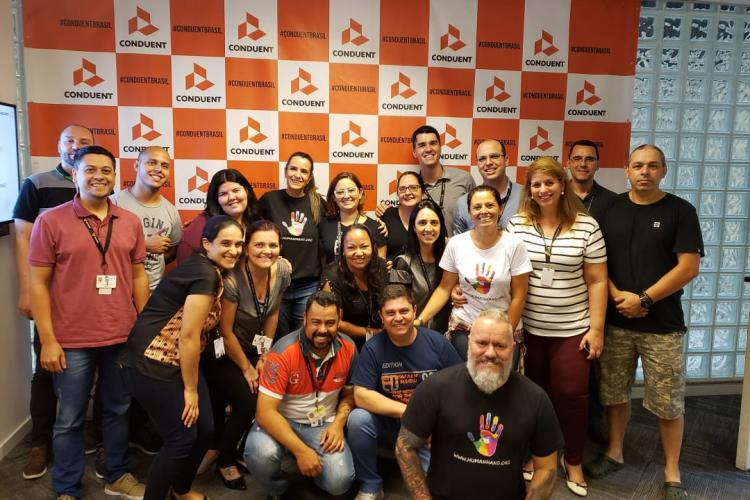
\includegraphics[width=1\textwidth]{figuras/mama.jpg}
\end{figure}
%---------------------------------------------------------------------------------------
\chapter{Contrato estabelecido}
Apesar do contrato só se estabelecer nesta etapa, a empresa já possui um vínculo de emprego e já oferece remuneração desde a etapa anterior (de treinamento).

Após a conclusão de todas as etapas do processo ja foram selecionados os melhores candidatos para exercer a função em questão. A etapa final do processo seletivo seria o estabelecimento do contrato com início de 3 meses no período de experiência, que seria o primeiro passo para a pessoa ser admitida dentro da cultura empresarial e do ambiente de trabalho. Realizadas todas as etapas anteriores, as pessoas selecionadas já possuem as capacitações necessárias para trabalhar na empresa e recebem a oportunidade de iniciar ou continuar suas carreiras.

Assim se inicia a jornada do trabalhador recém-admitido em um novo local de trabalho, com novas pessoas, novas funções e principalmente novas possibilidades.

\begin{figure}[h]

\centering

\includegraphics[width=1\textwidth]{figuras/mao.jpg}
\end{figure}


\section{Conclusão}

O desenvolvimento desse trabalho evidenciou alguns dos principais aspectos positivos e negativos identificados no processo seletivo da \emph{Conduent}, e, de maneira geral, pode-se constatar que há nele sinais da crescente centralidade no indivíduo adotada por empresas no mundo contemporâneo, porém, ainda existem algumas fragilidades nas etapas que não proporcionam total valorização do indivíduo.

Observa-se que, ao disponibilizar vagas online, a empresa conseguiu atrair um público diverso, mas notou-se a falta de estrutura para um grupo que ainda enfrenta diversas dificuldades de inserção no mercado de trabalho: as Pessoas Com Deficiência (PCD). Dado o ideal de diversidade preconizado pela organização, essa inclusão mostra-se benéfica por contribuir para que mais indivíduos tenham oportunidades no mercado de trabalho. 

Já em relação aos testes realizados do início ao fim da entrevista, tem-se que havia neles algumas disparidades em relação ao real nível de conhecimento demandado pela função de Analista de Suporte Bilíngue Júnior - ora o conhecimento era menor, ora maior que o necessário - e a falta de testes e dinâmicas indivíduais e/ou em grupo que pudessem demonstrar melhor o perfil psicológico do candidato. Essa análise acabou por ficar restrita a uma única entrevista presencial e, dado que a função demandava um bom nível de manipulação das \emph{Soft Skills} também abordadas nesse trabalho, existe o risco de que as expectativas e potencial do candadito poderiam encontrar-se desniveladas, causando, assim, frustração ou insatisfação nesse.

No que tange o treinamento após aprovação nas etapas anteriores, focava-se no autodesenvolvimento das habilidades técnicas e emocionais de cada indivíduo e buscava mostrar a esses as oportunidades de crescimento que a empresa fornecia. Nesse ponto, o conforto gerado pelo ambiente criado caracteriza-se como um dos principais pontos positivos do processo, pois durante ele, a centralidade no indivíduo se manisfestou da maneira visível. Contudo, a prova final, ainda seguia um modelo pré-pronto e, isolada, desconsiderava aspectos psicológicos do indivíduo, demonstrando que, apesar de grande valorização do humano durante o perído de treinamento, a habilidade técnica por vezes teria maior peso. 

Diante de tais pontos-chave e dos demais abordados no trabalho, conclui-se que o processo de seleção da  \emph{Conduent} do Brasil ainda não está integralmente voltado ao indivíduo, e tal como muitas empresas, necessita de readaptações e reformulações de etapas e testes para que isso ocorra. 

As maneiras pelas quais essas reestruturações podem ocorrer são diversas, mas observa-se um ponto em comum que poderia ser de grande auxilio para isso: uma maior diversificação na análise das \emph{Hard Skills} e personalização na análise do perfil psicológico dos candidatos, sempre objetivando entender se a função contribuirá para que esse alcance autorrealização.

Assim, ao ter-se maior enfoque na compreensão de se a empresa encaixa-se no perfil e objetivos do candidato, temos que frustrações são evitadas por ambas as partes e a nitidez na relação entre empregador e emprego é estabelecida desde seu início. 

Um exemplo de personalização e diversificação adotado por algumas empresas centradas no indíviduo é a aplicação de um treinamento antes mesmo da análise elimitória de currículos. 

Dar a cada indivíduo interessado a oportunidade de demonstrar suas capacidades em maior tempo tanto de habilidades técnicas quanto interpessoais mostra-se como uma alternativa justa ao modelo de entrevista ainda predominante que valoriza as individualidades de cada candidato e facilita o seu autorrealizar individual. 

Isto posto, conclui-se que a área de recrutamento é dinâmica e tende criar mais ferramentas e alternativas para que o ser humano seja cada vez mais valorizado. O que torna necessário e benéfico o consequente enfoque das organizações em cada um dos indivíduos que integram seu time. 

| Bibliografia |

\end{document}
